\documentclass[tikz,border=2pt]{standalone}
\usepackage[T1]{fontenc}
\usepackage{helvet,amsmath,amssymb,fix-cm}
\renewcommand{\familydefault}{\sfdefault}
\usetikzlibrary{arrows.meta,calc,positioning,fit,backgrounds,decorations.pathreplacing,shapes.geometric}
\definecolor{ink}{HTML}{243343}
\definecolor{physical}{HTML}{3478A3}
\definecolor{semantic}{HTML}{B27C26}
\definecolor{feasible}{HTML}{248679}
\definecolor{decode}{HTML}{75609D}
\definecolor{fault}{HTML}{BA5554}
\definecolor{muted}{HTML}{6F7D88}
\tikzset{
  every node/.style={font=\fontsize{9}{10.8}\selectfont,text=ink},
  edge/.style={-{Stealth[length=1.8mm,width=1.25mm]},line width=.6pt,draw=ink},
  param/.style={-{Stealth[length=1.7mm]},line width=.6pt,draw=decode,dashed},
  link/.style={line width=.8pt,draw=physical},
  reject/.style={line width=.7pt,draw=fault,dashed},
  panel/.style={rounded corners=2pt,draw=muted!45,line width=.45pt,fill=white},
  box/.style={rounded corners=2pt,draw=physical!70,line width=.55pt,fill=physical!6,align=center,inner sep=3pt},
  sem/.style={box,draw=semantic!70,fill=semantic!8},
  gate/.style={box,draw=feasible!70,fill=feasible!7},
  dec/.style={box,draw=decode!70,fill=decode!7},
  tinylabel/.style={font=\fontsize{8}{9.4}\selectfont},
  smalllabel/.style={font=\fontsize{8.5}{10}\selectfont},
  heading/.style={font=\bfseries\fontsize{10}{11.5}\selectfont,anchor=north west},
  dot/.style={circle,minimum size=.43cm,inner sep=0pt,draw=physical,fill=white,line width=.8pt,font=\bfseries\fontsize{9}{10}\selectfont},
  receiver/.pic={\draw[draw=physical,line width=.8pt] (0,0)--(0,.58) (-.17,0)--(.17,0) (-.15,.39)--(0,.58)--(.15,.39);
    \draw[draw=physical!70,line width=.55pt] (-.2,.56) arc[start angle=160,end angle=200,radius=.23];
    \draw[draw=physical!70,line width=.55pt] (.2,.40) arc[start angle=-20,end angle=20,radius=.23];},
}
\begin{document}
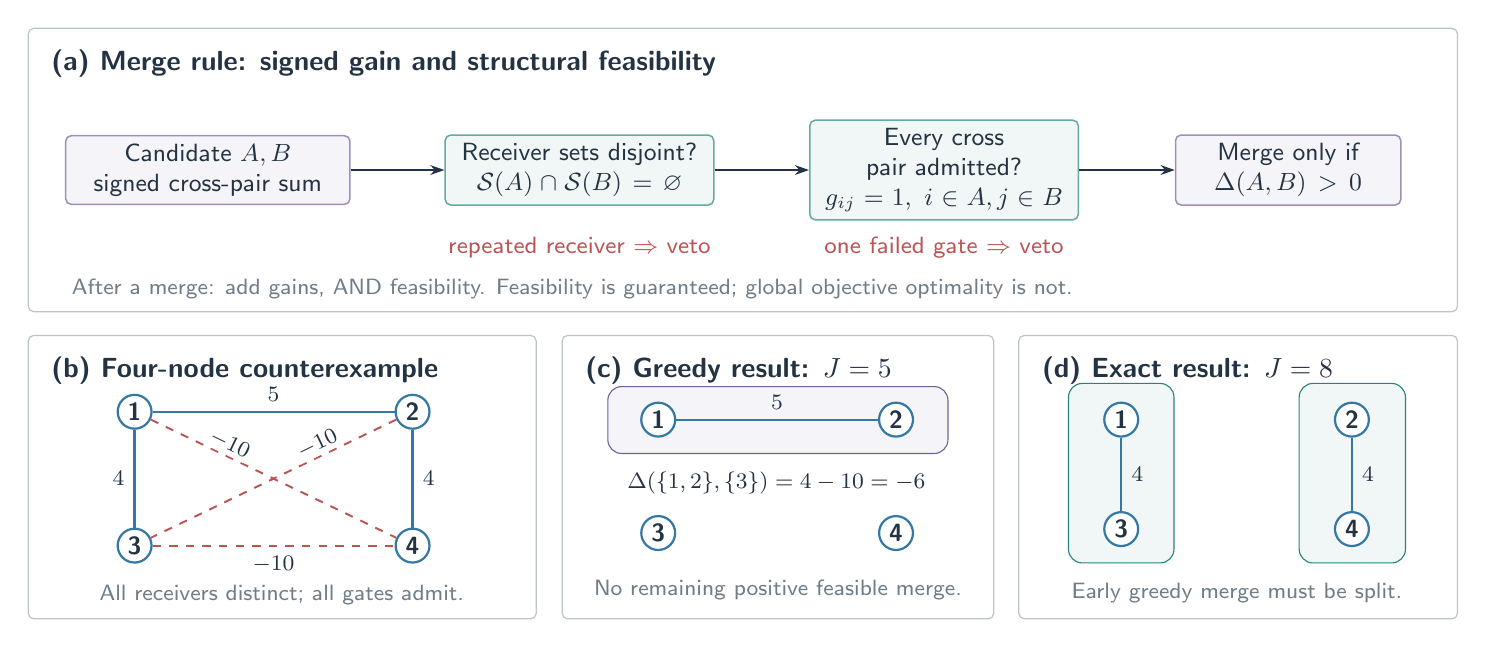
\begin{tikzpicture}[x=1cm,y=1cm]
\draw[panel] (0,3.9) rectangle ++(18.15,3.6);
\node[heading] at (0.17,7.35) {(a) Merge rule: signed gain and structural feasibility};
\draw[panel] (0,0) rectangle ++(6.45,3.6);
\node[heading] at (0.17,3.45) {(b) Four-node counterexample};
\draw[panel] (6.78,0) rectangle ++(5.48,3.6);
\node[heading] at (6.95,3.45) {(c) Greedy result: $J=5$};
\draw[panel] (12.58,0) rectangle ++(5.57,3.6);
\node[heading] at (12.75,3.45) {(d) Exact result: $J=8$};

\node[dec,text width=3.40cm,minimum height=.85cm] (candidate) at (2.28,5.70)
 {Candidate $A,B$\\signed cross-pair sum};
\node[gate,text width=3.20cm,minimum height=.85cm] (rxcheck) at (7.00,5.70)
 {Receiver sets disjoint?\\$\mathcal S(A)\cap\mathcal S(B)=\varnothing$};
\node[gate,text width=3.20cm,minimum height=.85cm] (allcheck) at (11.63,5.70)
 {Every cross pair admitted?\\$g_{ij}=1,\ i\in A,j\in B$};
\node[dec,text width=2.65cm,minimum height=.85cm] (accept) at (16.00,5.70)
 {Merge only if\\$\Delta(A,B)>0$};
\draw[edge] (candidate)--(rxcheck);\draw[edge] (rxcheck)--(allcheck);\draw[edge] (allcheck)--(accept);
\node[smalllabel,text=fault] at (7.00,4.71) {repeated receiver $\Rightarrow$ veto};
\node[smalllabel,text=fault] at (11.63,4.71) {one failed gate $\Rightarrow$ veto};
\node[tinylabel,text=muted,anchor=west] at (.43,4.19)
 {After a merge: add gains, AND feasibility. Feasibility is guaranteed; global objective optimality is not.};
\node[dot] (n1) at (1.35,2.63) {1};\node[dot] (n2) at (4.88,2.63) {2};
\node[dot] (n3) at (1.35,.93) {3};\node[dot] (n4) at (4.88,.93) {4};
\draw[link] (n1)--node[above,tinylabel] {$5$} (n2);
\draw[link] (n1)--node[left,tinylabel] {$4$} (n3);
\draw[link] (n2)--node[right,tinylabel] {$4$} (n4);
\draw[reject] (n3)--node[below,tinylabel] {$-10$} (n4);
\draw[reject] (n1)--node[pos=.30,above,sloped,tinylabel,fill=white,inner sep=1pt] {$-10$} (n4);
\draw[reject] (n2)--node[pos=.30,above,sloped,tinylabel,fill=white,inner sep=1pt] {$-10$} (n3);
\node[tinylabel,text=muted] at (3.22,.30) {All receivers distinct; all gates admit.};

\draw[draw=decode,fill=decode!7,rounded corners=5pt] (7.36,2.10) rectangle (11.68,2.95);
\node[dot] (g1) at (8.00,2.53) {1};\node[dot] (g2) at (11.02,2.53) {2};
\draw[link] (g1)--node[above,tinylabel] {$5$} (g2);
\node[dot] at (8.00,1.09) {3};\node[dot] at (11.02,1.09) {4};
\node[tinylabel] at (9.50,1.73) {$\Delta(\{1,2\},\{3\})=4-10=-6$};
\node[tinylabel,text=muted] at (9.52,.37) {No remaining positive feasible merge.};

\draw[draw=feasible,fill=feasible!7,rounded corners=5pt] (13.21,.71) rectangle (14.55,2.99);
\draw[draw=feasible,fill=feasible!7,rounded corners=5pt] (16.14,.71) rectangle (17.49,2.99);
\node[dot] (e1) at (13.88,2.53) {1};\node[dot] (e2) at (16.81,2.53) {2};
\node[dot] (e3) at (13.88,1.14) {3};\node[dot] (e4) at (16.81,1.14) {4};
\draw[link] (e1)--node[right,tinylabel] {$4$} (e3);
\draw[link] (e2)--node[right,tinylabel] {$4$} (e4);
\node[tinylabel,text=muted] at (15.35,.33) {Early greedy merge must be split.};
\end{tikzpicture}
\end{document}
